
\section{maincontent}

\begin{frame}
\frametitle{Femtosecond Reduction of Atomic Scattering Factors Triggered by 
Intense X-Ray Pulse \small (Phys. Rev. Lett. \textbf{131}, 163201 (2023))}
\framesubtitle{X-Ray diffraction  (XRD) fundamentals and important definition}


\footnotesize
\begin{textblock*}{200pt}(30pt,70pt)
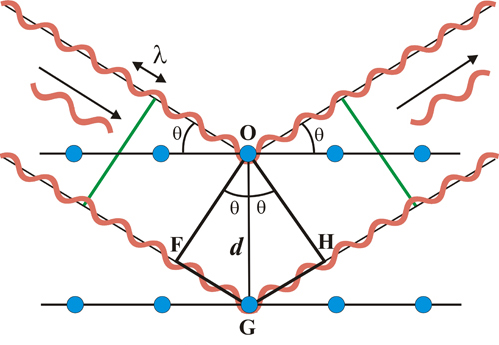
\includegraphics[scale=.20]{images/bragg-1.jpg}
\includegraphics[scale=.20]{images/rayleigh.png}

\begin{align}
2d\sin\theta = n\lambda
\end{align}
\end{textblock*}
 
\begin{textblock*}{400pt}(30pt,60pt)
\begin{itemize}
\footnotesize
\item Elastic scattering and Bragg's law
\end{itemize}
\end{textblock*}


\begin{textblock*}{400pt}(30pt,165pt)
\begin{itemize}
\footnotesize
\item Auger electron
\end{itemize}
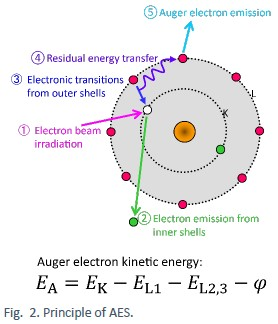
\includegraphics[scale=.40,trim={0 50 0 0}, clip]{images/img_aes2.jpg}
\end{textblock*}


\begin{textblock*}{200pt}(230pt,60pt)
\begin{itemize}
\item Miller indexes
\end{itemize}
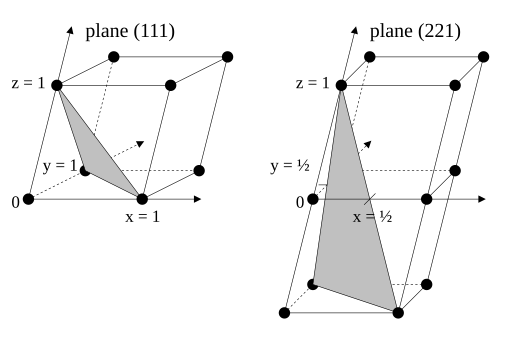
\includegraphics[scale=.20]{images/miller_plan.png}
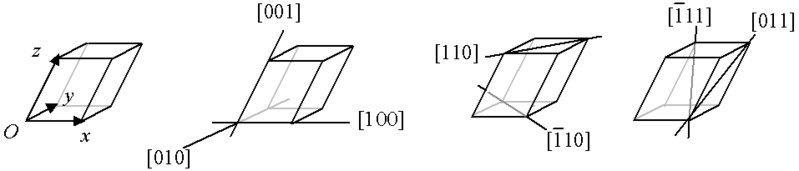
\includegraphics[scale=.20]{images/miller_direction_exemples.png}
\begin{align}
\footnotesize
\boldsymbol{\rm g}_{hkl} = h\boldsymbol{b}_1 
+ k\boldsymbol{b}_2  + l\boldsymbol{b}_3 
\end{align}
\begin{align}
\footnotesize
d = 2\pi/|\boldsymbol{\rm g}_{hkl}|
\end{align}
\end{textblock*}

\end{frame}


\begin{frame}
\frametitle{Femtosecond Reduction of Atomic Scattering Factors Triggered by 
Intense X-Ray Pulse \small (Phys. Rev. Lett. \textbf{131}, 163201 (2023))}
\framesubtitle{Atomic scattering factor and X-ray diffraction intensity}


\footnotesize
%\begin{textblock*}{200pt}(250pt,60pt)
%\begin{itemize}
%\item 3 steps model
%
\includegraphics[scale=.20]{images/Color-online-Schematic-representation-of-the-dominant-physical-mechanisms-behind.png}
%\end{itemize}
%\end{textblock*}
 
\begin{textblock*}{200pt}(30pt,60pt)
\begin{itemize}
\footnotesize
\item Scattering vector
\begin{equation}
Q = 2k\sin\theta
\end{equation}
\item Atomic form factor
\begin{equation}
f(\boldsymbol{Q}) = \int \rho(\boldsymbol{r})
  e^{i\boldsymbol{Q}\cdot\boldsymbol{r}} d^3\boldsymbol{r}
\end{equation}

\item total scattered wave and scattered intensity (identical atoms)
\begin{align}
\boldsymbol{\Psi}_s(\boldsymbol{Q}) & = f(\boldsymbol{Q})\sum_{j=1}^N 
   e^{-i\boldsymbol{Q}\cdot\boldsymbol{r}_j} \\
I(\boldsymbol{Q}) 
& = \boldsymbol{\Psi}_s(\boldsymbol{Q})\boldsymbol{\Psi}_s^{*}(\boldsymbol{Q}) 
\sim \left| f(\boldsymbol{Q})\right|^2
\end{align}


\end{itemize}
\end{textblock*}


%\begin{textblock*}{100pt}(330pt,210pt)
%\begin{align}
%\footnotesize
%U_p = \frac{F_0^2}{4\omega^2}, \hspace{20pt} 
%\gamma = \sqrt{\frac{I_p}{2U_p}}\nonumber
%\end{align}
%\end{textblock*}

\end{frame}







\begin{frame}
\frametitle{Femtosecond Reduction of Atomic Scattering Factors Triggered by 
Intense X-Ray Pulse \small (Phys. Rev. Lett. \textbf{131}, 163201 (2023))}
\framesubtitle{Experimental setup}

\begin{textblock*}{100pt}(280pt,70pt)

\includegraphics[scale=.33, trim={0 0 0 0}, clip]{images/medium1.png}
\end{textblock*}

\small
\begin{textblock*}{250pt}(30pt,60pt)
\begin{itemize}
\footnotesize
\item Material is silicon ${\rm Si}\;(Z=14)$  
\item Fluence in the range $ 1.3\times 10^{2} - 3.0\times 10^{5}\,\rm J/cm^2$
\item Intensity in the range of  
$2.1\times 10^{16} - 4.6\times 10^{19}\,\rm W/cm^2$
\item Pulse duration is  $6 \leqslant 10\,\rm fs$
\item Induced atomic disordering becomes prominent at 
$\sim 20\,\rm fs$\footnote{\tiny Ziaja \textit{et al.}, Phys. Rev. B \textbf{64}, 2004}
\item SACLA beamline 3 frequency is  $11.5\,\rm keV$
\end{itemize}
\end{textblock*}

\begin{textblock*}{100pt}(280pt,180pt)
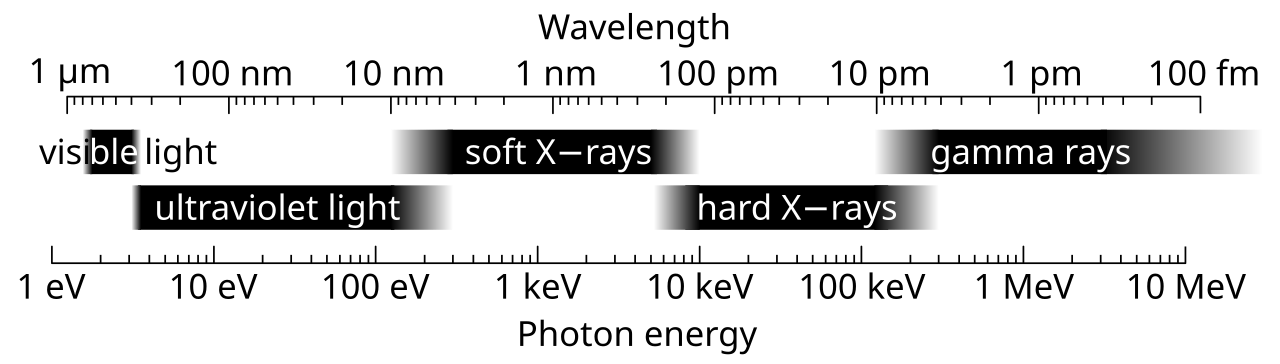
\includegraphics[scale=.13, trim={0 0 0 0}, clip]{images/X-ray_range.png}
\end{textblock*}


\end{frame}


\begin{frame}
\frametitle{Femtosecond Reduction of Atomic Scattering Factors Triggered by 
Intense X-Ray Pulse \small (Phys. Rev. Lett. \textbf{131}, 163201 (2023))}
\framesubtitle{Question}


\footnotesize
%\begin{textblock*}{200pt}(250pt,60pt)
%\begin{itemize}
%\item 3 steps model
%
\includegraphics[scale=.20]{images/Color-online-Schematic-representation-of-the-dominant-physical-mechanisms-behind.png}
%\end{itemize}
%\end{textblock*}
 
\begin{textblock*}{400pt}(30pt,60pt)
\begin{align}
I(\boldsymbol{Q})  \sim \left| f(\boldsymbol{Q})\right|^2 \nonumber
\end{align}
\begin{itemize}
\item If a reduction of $I(\boldsymbol{Q})$ at very high intensity
it means that $f(\boldsymbol{Q})$ has been reduced..
\begin{itemize}
\footnotesize
\item[$\bullet$] which in turn, means that $\boldsymbol{Q}$ 
varied significantly to make that happen...
\item[$\bullet$] right?
\end{itemize}
\item Or is the reduction linked to a change in the structure of the media
at such a high intensity?
\end{itemize}
\end{textblock*}


%\begin{textblock*}{100pt}(330pt,210pt)
%\begin{align}
%\footnotesize
%U_p = \frac{F_0^2}{4\omega^2}, \hspace{20pt} 
%\gamma = \sqrt{\frac{I_p}{2U_p}}\nonumber
%\end{align}
%\end{textblock*}

\end{frame}





\begin{frame}
\frametitle{Femtosecond Reduction of Atomic Scattering Factors Triggered by 
Intense X-Ray Pulse \small (Phys. Rev. Lett. \textbf{131}, 163201 (2023))}
\framesubtitle{XRD intensity profiles of $\rm Si$ at high peak intensities}

\begin{textblock*}{100pt}(300pt,52pt)

\includegraphics[scale=.38]{images/medium2.png}
\end{textblock*}

\small
\begin{textblock*}{250pt}(30pt,60pt)
\begin{itemize}
\footnotesize
\item No suppression seen for the lower intensities in (a) and (b)
\begin{itemize}
\footnotesize
\item[$\bullet$] XFEL pulses with intensities up to $\sim 10^{18}\,\rm W/cm^2$
do not change the atomic scattering factors
\end{itemize}
\item Suppression identified for $I=(4.6\pm 1.2)\times 10^{19}\,\rm W/cm^2$
\begin{itemize}
\footnotesize
\item[$\bullet$] This indicates structural and/or electronic damage
\end{itemize}
\vspace{20pt}
\item For quantitatively evaluating the suppression
\begin{itemize}
\footnotesize
\item[$\bullet$] Fitting the profiles in the vicinity of diffraction peaks
\item[$\bullet$] Substraction of the background
\item[$\bullet$] Fitting each diffraction peak by a gaussian function 
\end{itemize}
\end{itemize}
\end{textblock*}


\end{frame}



\begin{frame}
\frametitle{Femtosecond Reduction of Atomic Scattering Factors Triggered by 
Intense X-Ray Pulse \small (Phys. Rev. Lett. \textbf{131}, 163201 (2023))}
\framesubtitle{Diffraction efficiency and scattering vector}

\begin{textblock*}{100pt}(60pt,60pt)
\input{tables/tab1.tab}
\end{textblock*}

\small
\begin{textblock*}{400pt}(30pt,130pt)
\begin{itemize}
\footnotesize
\item The background subtracted and the peak is fitted by a gaussian  
\item The scattering vector $Q$ is then evaluated as
\begin{equation}
Q = \frac{4\pi \sin \theta}{\lambda}
\end{equation}
\begin{itemize}
\footnotesize
\item[$\bullet$] The diffraction efficiency not depending much on $Q$
\item[$\bullet$] The latter suggest that atomic disordering (caused by $Q$) 
was not present
\end{itemize}
\item So the reduction of diffraction intensity has to be caused 
by femtosecond change in atomic scattering factors due to the electronic excitation induced by the pulse
\end{itemize}
\end{textblock*}


\end{frame}




\begin{frame}
\frametitle{Femtosecond Reduction of Atomic Scattering Factors Triggered by 
Intense X-Ray Pulse \small (Phys. Rev. Lett. \textbf{131}, 163201 (2023))}
\framesubtitle{XMDYN molecular dynamic simulation}

\begin{textblock*}{100pt}(280pt,70pt)

\includegraphics[scale=.33]{images/medium3.png}
\end{textblock*}

\small
\begin{textblock*}{250pt}(30pt,60pt)
\begin{itemize}
\footnotesize
\item $I_{\rm eff}^{hkl}$ evaluated for different numerical $I_{\rm high}^{hkl}$
\item Fig. 3(a) : $I=1.0\times 10^{20}\,\rm W/cm^2$ reproduces the
previous trend
\item Fig. 3(b) : Simulated root mean square atomic displacement during the irradiation $${\rm RMSD} = \sqrt{\frac{1}{N}\sum_{i=1}^N \delta_i}$$
\begin{itemize}
\footnotesize
\item[$\bullet$] Negligible against interatomic distance
\end{itemize}
\item Fig. 3 : (c) Relative ion populations and 
(d) locations of the holes during the interaction with the pulse
\vspace{10pt}
\item Thus, suppression of diffraction intensity is caused by the reduction 
of the atomic scattering factors for
$I = 4.6\times 10^{19}\,\rm W/cm^2$

\end{itemize}
\end{textblock*}

\end{frame}

